% !TEX root = ../main.tex
% ---------------------------------------------------------------
% GOALS
% ---------------------------------------------------------------



\chapter[Obiettivi]{Obiettivi}\label{chap4:Goals}
Allo stato dell'arte, riassunto nella tabella \ref{letteratura}, sono presenti molti lavori di classificazione del Freezing, usando principalmente 2 classi, ossia noFOG, che corrisponde ad attività definite normali del paziente, e FOG, ossia un blocco motorio. Uno studio ha cercato di introdurre una nuova classe, intermedia tra le due, che é stata chiamata preFOG. Questa rappresenta una fase transitoria da uno stato di noFOG ad un'occorrenza di FOG. Identificare tale classe permetterebbe di prevedere i Freezing del paziente e quindi permettergli di non bloccarsi attraverso uno stimolo, uditorio o visivo.\\
Gli studi condotti finora, inoltre, utilizzano dei dataset composti da dati ricavati tramite accelerometri ed etichettati manualmente da dottori. Non é stato ancora presentato un approccio che tenti di sostituire il lavoro di etichettatura dei dati del medico.\\
La tesi proposta si prefigge lo scopo di presentare un approccio non supervisionato per l'etichettatura dei dati provenienti da accelerometri senza l'ausilio del medico ed usare un approccio di classificazione per identificare le occorrenze di preFOG al fine di prevedere i Freezing.\\
\begin{tikzpicture}
\node [mybox] (box){%
	\begin{minipage}{.96\textwidth}
		Gli obiettivi della tesi quindi sono:
			\begin{itemize}
				\item Studio dei dati tramite le classi fornite dal medico;
				\item Usare un approccio non supervisionato per l'etichettatura dei dati e fornire uno studio di divisione degli intervalli temporali dei dati;
				\item Classificare i dati per identificare le occorrenze di preFOG e fornire uno stimolo sensoriale per evitare FOG.
			\end{itemize}
	\end{minipage}
};
\end{tikzpicture}%
%Il lavoro condotto, partendo da dati raccolti dagli assi x,y,z di più accelerometri, verifica la presenza di una nuova tipologia di classe, che chiameremo preFOG, dei dati e conduce uno studio algoritmico non supervisionato su feature ed intervalli temporali sui dati per etichettare tali dati, sostituendo in tale modo il lavoro del medico. Inoltre, introduce un metodo di classificazione dei dati stessi, al fine di identificare tale classe per evitare le occorrenze del Freezing.\\
%\begin{tikzpicture}
%\node [mybox] (box){%
%	\begin{minipage}{.96\textwidth}
%	Quello che, dunque, si vuole studiare è innanzitutto l'esistenza di una nuova classe chiamata preFoG e che sia divisa da quelle di FoG e noFoG. Una volta verificato questo, si vuole sviluppare un procedimento di riconoscimento non supervisionato di etichette delle varie classi attraverso algoritmi di clustering, sostituendo cosí il medico nella prima fase di test. Sfruttando tale intervallo, inoltre, si vuole tentare un approccio di classificazione per identificare le occorrenze di preFOG.
%	\end{minipage}
%};
%\end{tikzpicture}%
\\ La figura \ref{FlussoTesiGenerale} rappresenta il flusso degli obiettivi della tesi. La fase 1, da dati di accelerometri, vuole valutare, tramite uno studio dei dati, la distinzione tra le varie classi, specialmente quella del preFOG. 
La fase 2, usando tale informazione, applica un approccio non  supervisionato al fine di etichettare i dati senza l'ausilio di un medico e conduce uno studio sugli intervalli temporali, ossia il modo migliore per dividere i dati di ingresso degli accelerometri. La fase 3, usando le informazioni sulle finestre di suddivisione temporale dei dati della fase precedente, si pone l'obiettivo di usare un classificatore per generare uno stimolo sensoriale al fine di evitare FOG.
\begin{figure}[]
	\centering
	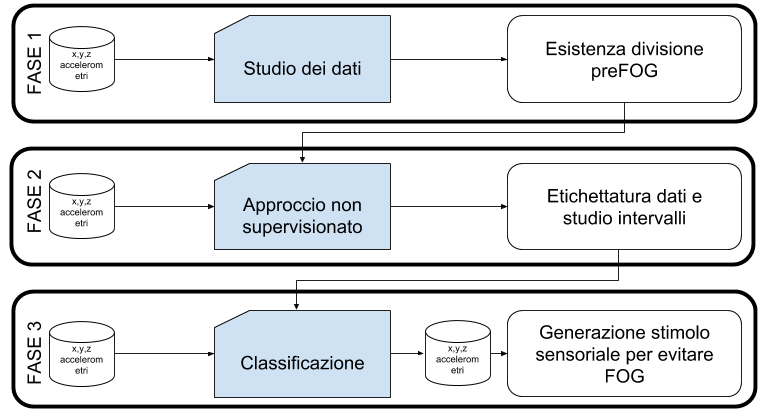
\includegraphics[width=1\textwidth]{images/FlussoTesiGenerale.png}
	\caption{Rappresentazione del flusso generale della tesi}
	\label{FlussoTesiGenerale}
\end{figure}
